\documentclass[11pt]{article}
\usepackage{geometry, titlesec}
\usepackage[parfill]{parskip}
\usepackage[italicdiff]{physics}
\usepackage{amsfonts, amsthm}
\usepackage[cm]{fullpage}
\usepackage{fancyhdr}
\usepackage{enumitem}
\usepackage{xcolor, soul}
\usepackage{graphicx}
\usepackage[export]{adjustbox}
\usepackage{siunitx}
%\allowdisplaybreaks

\renewcommand{\thesubsection}{\thesection.\alph{subsection}}
\setenumerate[1]{label={(\alph*)}}

\makeatletter
\renewcommand*\env@cases[1][1.2]{%
  \let\@ifnextchar\new@ifnextchar
  \left\lbrace
  \def\arraystretch{#1}%
  \array{@{}l@{\quad}l@{}}%
}
\makeatother
 
\renewcommand{\footrulewidth}{.2pt}
%\setlist[enumerate]{leftmargin=*}
\pagestyle{fancy}
\fancyhf{}
\rhead{Physics 132-B}
\lhead{\textbf{Homework 5 Solutions}}
%\rhead{A--De Discussion}
\setlength{\headheight}{11pt}
\setlength{\headsep}{11pt}
\setlength{\footskip}{24pt}
\lfoot{\today}
\rfoot{\thepage}

\titleformat{\subsection}[runin]{\normalfont\large\bfseries}{\thesubsection}{1em}{}
\newcommand{\refeq}[1]{(\ref{#1})}

\newcommand{\beq}{\begin{equation*}}
\newcommand{\eeq}{\end{equation*}}

\newcommand{\beqn}{\begin{equation}}
\newcommand{\eeqn}{\end{equation}}

\newcommand{\blg}{\begin{align*}}
\newcommand{\elg}{\end{align*}}


\newenvironment{statement}
{
%    \color{gray}
    \ignorespaces
}
{
%    \smallskip
}

\newenvironment{problem}
{
    \color{darkgray}
    \ignorespaces
}

\newenvironment{solution}
{
    \paragraph{Solution.}
    \ignorespaces
}
{
    \bigskip
}

\renewcommand{\vec}[1]{\mathbf{#1}}
\renewcommand{\theequation}{\Alph{equation}}


\begin{document}

\newcommand{\Vab}{V_{ab}}
\newcommand{\cE}{\mathcal{E}}
\newcommand{\sicE}{\SI{12.0}{\volt}}
\newcommand{\sir}{\SI{0.400}{\ohm}}
\newcommand{\siP}{\SI{80.0}{\watt}}
	

\paragraph{Problem 25.58}
\begin{problem}
	A resistor with resistance $R$ is connected to a battery that has emf \sicE and internal resistance $r = \sir$.  For what two values of $R$ will the power in the resistor be \siP?
\end{problem}

\begin{solution}
	The power $P$ delivered to a resistor is
	\beqn \tag{25.18} \label{25.18}
		P = I^2 R,
	\eeqn
	where $I$ is the current through the resistor and $R$ its resistance.  We can find the current from
	\beqn \tag{25.17} \label{25.17}
		\Vab = \cE - I r,
	\eeqn
	where $\Vab$ is the voltage difference across the resistor, $\cE$ is the emf of the battery, and $r$ its internal resistance.  We also know that
	\beqn \tag{25.11} \label{25.11}
		\Vab = I R.
	\eeqn
	Substituting \refeq{25.11} into \refeq{25.17}, we get
	\beq
		IR = \cE - Ir
		\implies
		\cE = I (R + r)
		\implies
		I = \frac{\cE}{R + r}.
	\eeq
	Now we can substitute this result into \refeq{25.18} and solve for $R$:
	\begin{align*}
		P = \frac{\cE^2}{(R + r)^2} R
		&\implies
		\cE^2 R = P (R^2 + 2 R r + r^2)
		\implies
		0 = P R^2 + (2P r - \cE^2) R + P r^2 \\
		&\implies
		R = \frac{\cE^2 - 2 P r \pm \sqrt{(2P r - \cE^2)^2 - 4 P^2 r^2}}{2 P}
	\end{align*}
	Plugging in our numerical values for $r$, $P$, and $\cE$, and recalling that $\SI{1}{\watt} = \SI{1}{\square\volt\per\ohm}$, we get
	\begin{align*}
		R &= \frac{(\sicE)^2 - 2 (\siP) (\sir) \pm \sqrt{[2 (\siP) (\sir) - (\sicE)^2]^2 - 4 (\siP)^2 (\sir)^2}}{2 (\siP)} \\
		&= \frac{\SI{80.0}{\square\volt} - \pm \sqrt{(\SI{80}{\square\volt})^2 - (\SI{64}{\square\volt})}}{\SI{160}{\square\volt\per\ohm}}
		= \frac{\SI{80.0}{\square\volt} \pm \sqrt{\SI{2306}{\volt^4}}}{\SI{160}{\square\volt\per\ohm}}
		= \frac{80.0 \pm 48.0}{160} \,\si{\ohm}
		= (0.50 \pm 0.30) \,\si{\ohm} \\
		&= \begin{cases}
			{\color{blue} \SI{0.80}{\ohm}}, \\
			{\color{blue} \SI{0.20}{\ohm}}.
		\end{cases}
	\end{align*}
\end{solution}

%\clearpage

\newcommand{\Iq}{I_1}
\newcommand{\Iw}{I_2}
\newcommand{\Ie}{I_3}

\begin{minipage}[b]{0.75\textwidth}
\paragraph{Exercise 26.26}
\begin{problem}
	In the circuit shown in Fig.~E26.28, find
	\begin{enumerate}
		\item the current in each branch, and
		\item the potential difference $\Vab$ of point $a$ relative to point $b$.
	\end{enumerate}
\end{problem}
\end{minipage}%
\begin{minipage}{0.35\textwidth}
	%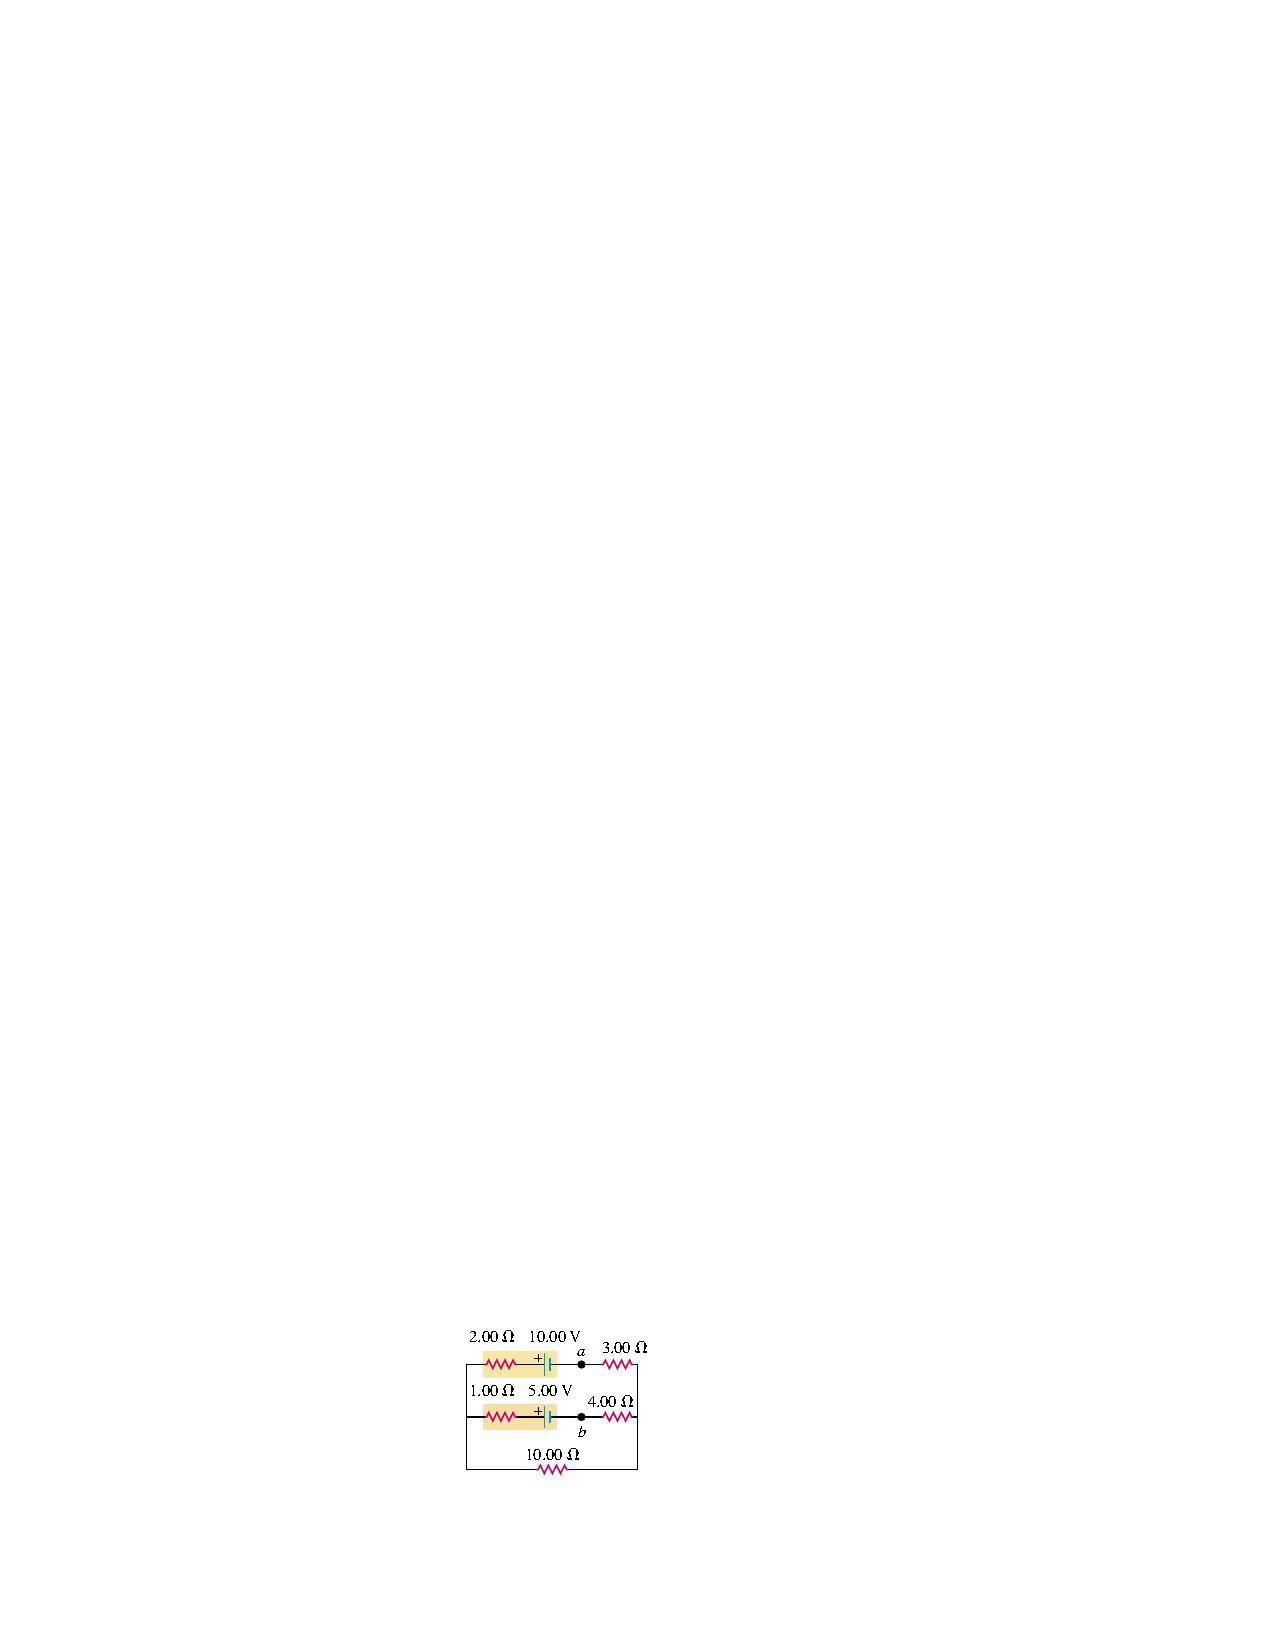
\includegraphics[width=\textwidth]{E26-26}
	\center \textbf{Figure \hl{E26.28}}
\end{minipage}

\begin{solution}
	\begin{enumerate}
		\item We need to use Kirchhoff's rules.  Since this circuit has more than one loop, we need to use both the junction rule,
		\beqn \tag{26.5} \label{26.5}
			\sum I = 0,
		\eeqn
		and the loop rule,
		\beqn \tag{26.6} \label{26.6}
			\sum V = 0.
		\eeqn
		Let's choose the current to be flowing to the right across the \SI{10.00}{\volt} battery, and start with the loop rule.  For the top loop, we have
		\beqn 
			0= \SI{10}{\volt} -\Iq (\SI{2}{\ohm}) - \Iq (\SI{1}{\ohm}) - \SI{5}{\volt} - \Iq (\SI{4}{\ohm}) - \Iq (\SI{3}{\ohm})
			= \SI{5}{\volt} - \Iq (\SI{10}{\ohm})
		\eeqn
	\end{enumerate}
\end{solution}

%
%\vfill
%
%
%\clearpage
%
%\begin{minipage}[b]{0.65\textwidth}
%%\paragraph{Problem 22.34}
%\paragraph{Problem 3}
%\begin{problem}
%	A cube has sides of length $L = \SI{0.350}{\meter}$.  One corner is at the origin~(Fig.~2).  The nonuniform electric field is given by ${\vE = (\SI{-5.64}{\newton\per\coulomb\per\meter})x \, \vec{\hat{i}} + (\SI{2.54}{\newton\per\coulomb\per\meter}) z \, \vec{\hat{k}}}$. \medskip
%	\begin{enumerate}
%		\item Find the electric flux through each of the six cube faces $S_1,\ S_2,\ S_3,\ S_4,\ S_5$, and $S_6$. \medskip
%		\item Find the total electric charge inside the cube.
%	\end{enumerate}
%\end{problem}
%\end{minipage}%
%\begin{minipage}[b]{0.65\textwidth}%\hspace{0.05\textwidth}%
%\begin{minipage}{0.3\textwidth}
%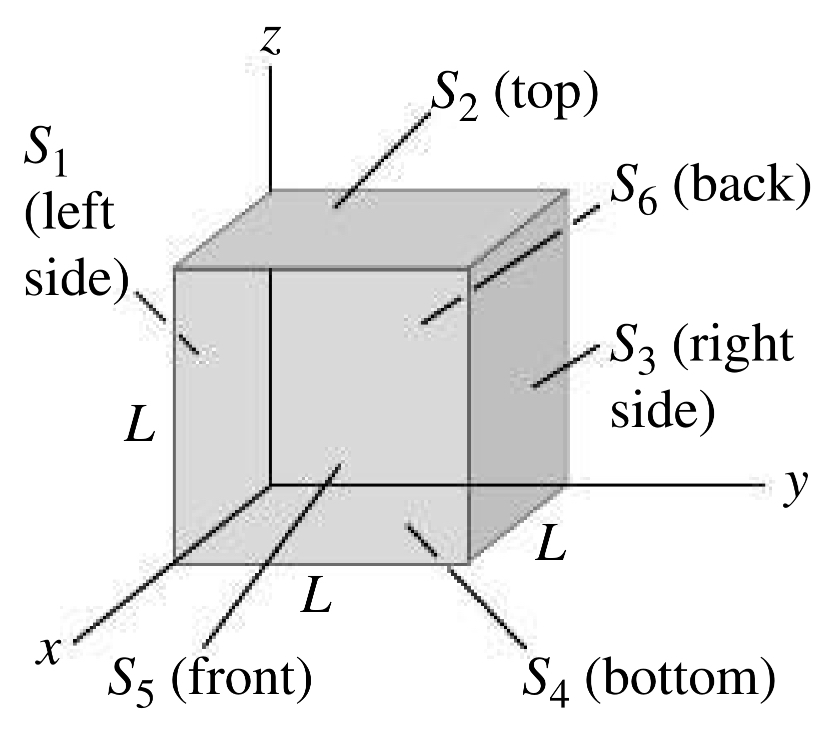
\includegraphics[width=\textwidth]{E22-6.jpeg}
%\center \textbf{Figure 3}
%\end{minipage}
%
%\vspace{-6\baselineskip}
%\vfill
%
%\paragraph{Problem 4}
%%\paragraph{Problem 24.11}
%\begin{problem}
%	A spherical capacitor contains a charge of \SI{3.10}{\nano\coulomb} when connected to a potential difference of \SI{240}{\volt}.  If its plates are separated by vacuum and the inner radius of the outer shell is \SI{4.40}{\centi\meter}, calculate
%	
%	\begin{enumerate}
%		\item the capacitance,
%		\item the radius of the inner sphere, and
%		\item the electric field just outside the surface of the inner sphere.
%	\end{enumerate}
%\end{problem}
%
%\vfill

\end{document}